\documentclass{article}

\usepackage[utf8]{inputenc}
\usepackage{amsmath}
\usepackage[uniquename=init,firstinits,backend=bibtex,sorting=none]{biblatex}
\usepackage{calc}
\usepackage{color}
\usepackage{gensymb}
\usepackage{graphicx}
\usepackage{listings}
\usepackage[numbered,framed]{mcode}
\usepackage[space]{grffile}
\usepackage{lineno}
%% hyperref manual advises loading this package last
\usepackage{hyperref}
\hypersetup{colorlinks=true,linkcolor=blue,citecolor=blue,breaklinks=true}

\definecolor{gray}{rgb}{0.9,0.9,0.9}

\lstloadlanguages{Matlab}
\lstset{basicstyle=\small,breaklines=true,frame=single,float,columns=fullflexible,numbers=left,stepnumber=2,backgroundcolor=\color{gray}}

\newcommand{\reals}{\mathbf R}

\linenumbers

\title{LCS Tool — An Algorithmic Introduction to Lagrangian Coherent 
Structures}

\author{Kristjan Onu \and Florian Huhn \and George Haller}

\addbibresource{main}

\begin{document}

\numberwithin{equation}{section}
\numberwithin{figure}{section}
\numberwithin{lstlisting}{section}
\numberwithin{table}{section}

\maketitle

\tableofcontents

\abstract{
We give an applied introduction to Lagrangian coherent structures (LCSs) using a computational engine we have programmed called LCS Tool. First, we review LCS theory that is based on variational calculus; this introduces elliptic and hyperbolic variational LCSs. Then we turn our attention to algorithms for computations conceived in accordance with the variational LCS theory. These algorithms are the foundation of LCS Tool. We conclude by explaining, with demonstration scripts, how to use LCS Tool to analyze three flow examples: a double gyre, a Bickley jet and an ocean dataset.
}

\section{Introduction}

LCSs are used in fluid dynamics to capture essential flow features and thereby simplify the description of complex fluid flows. Here we focus on analyzing two dimensional finite time turbulent flows. LCSs identify transport barriers, repelling and attracting structures and vortex boundaries. Application areas for LCSs include oceanic and atmospheric flows, biological applications\parencite{wilson09:_lagran_reynol,tallapragada11:_lagran}, aeronautics\parencite{tang10:_accur_lagran_hong_kong_inter_airpor} and mechanical systems\parencite{hadjighasem13:_detec_kam}.

The finite time Lyapunov exponent (FTLE) is one widely-used mathematical definition for LCSs. Despite its widespread use, examples where the FTLE fails to identify LCSs correctly are known\parencite{haller11:_lagran_coher_struc,norgard12:_secon_lagran_coher_struc}. To remedy these problems, variational calculus has been applied to material curve properties in the context of fluid mechanics. Thus we obtain a rigorous approach to LCS detection\parencite{haller11:_lagran_coher_struc,farazmand12:_comput_lagran,haller12:_geodes_theor_trans_barrier_two_dimen_flows,farazmand13:_attrac_lagran,haller13:_coher_lagran}. This article presents an algorithmic introduction to variational LCSs supported by a computational engine called LCS Tool\footnote{LCS Tool is available at: \url{https://github.com/jeixav/LCS-Tool}.}.

LCS Tool is a library of MATLAB functions that perform computations to identify LCSs in two dimensional finite time flows. LCS Tool aims to help scientists perform variational LCS calculations. The examples we present have been programmed into demonstration scripts. We encourage readers to download and execute these scripts after reading this article.

Other LCS software has been developed before; the list includes:
\begin{itemize}
\item \emph{MANGEN}\parencite{lekien03:_time}, calculates stability manifolds adaptively in two dimensional finite time velocity fields. Includes a graphical user interface and uses MPI for parallel calculations.
\item \emph{LCS MATLAB Kit}\parencite{dabiri09:_lmk} calculates the FTLE from velocity datasets. Includes a graphical user interface.
\item \emph{Newman}\parencite{toit10:_trans} calculates the FTLE in $N$ dimensions. Assists ridge extraction of FTLE fields. Supports analytic and dataset defined velocity definitions.
\item \emph{FlowVC}\parencite{shadden10:_flowvc} is a general purpose LCS platform for two and three dimensional datasets. Parallel calculations are supported with Open\-MP, CUDA and OpenCL.
\end{itemize}
These packages are based on the FTLE; the focus of LCS Tool and this article is to encourage and facilitate variational LCS analysis.

\section{Theory}

The fluid flows considered are defined in two dimensions by a velocity field:
\begin{align*}
\dot{\boldsymbol x} = \boldsymbol v(\boldsymbol x,t), && \boldsymbol x \in U \subset \reals^2, && t \in [t_-,t_+].
\end{align*}
Integration yields the flow map, defined between an initial time $t_0$ and a final time $t$ within $[t_-,t_+]$:
\[
F_{t_0}^t(\boldsymbol x_0) := \boldsymbol x(t,t_0,\boldsymbol x_0).
\]
The time interval used to detect LCSs is arbitrary; it can be the complete interval for which the flow is defined, or data is available, or it can be a sub-interval.

The right Cauchy-Green strain tensor measures Lagrangian strain in the velocity field and is defined:
\[
C_{t_0}^t(\boldsymbol x_0) = \left[D F_{t_0}^t(\boldsymbol x_0)\right]^T D F_{t_0}^t(\boldsymbol x_0).
\]
The eigenvalues of the Cauchy-Green strain tensor are denoted by $\lambda_{1,2}$ and the eigenvectors by $\boldsymbol \xi_{1,2}$. The eigenvalues satisfy $0 < \lambda_1 \leq \lambda_2$ and the eigenvectors satisfy $\boldsymbol \xi_1 \perp \boldsymbol \xi_2$.

\subsection{Elliptic LCS}
We find coherent Lagrangian vortices as closed orbits of one of the two vector fields
\begin{equation}
\boldsymbol \eta^{\lambda}_\pm = \sqrt{\frac{\lambda_2 - \lambda^2}{\lambda_2 - \lambda_1}} \boldsymbol \xi_1 \pm \sqrt{\frac{\lambda^2 - \lambda_1}{\lambda_2 - \lambda_1}} \boldsymbol \xi_2,
\label{eq:eta}
\end{equation}
which are a function of the eigenvalues and eigenvectors of $C_{t_0}^t(\boldsymbol x_0)$. Curves $\gamma$ that are trajectories of $\boldsymbol \eta^{\lambda}_\pm$ can be parametrized as $\boldsymbol r(s)$ with their arc length $s \in [0,\sigma]$. They are given by integrating
\begin{equation}
\boldsymbol r' \equiv \frac{d \boldsymbol r}{ds} = \boldsymbol \eta^{\lambda}_\pm(\boldsymbol r).
\label{eq:etafields}
\end{equation}

$\lambda$ is a free parameter close to unity that indicates the uniform stretching of the curve $\gamma$, i.e., each tangent vector $\boldsymbol r'(s)$ with length $l_{t_0}$ stretches by a factor $\lambda$ to length $l_{t}$ under the flow map:
\begin{gather*}
l_{t_0}(s) = \sqrt{\langle \boldsymbol r'(s), \boldsymbol r'(s) \rangle},\\
l_t(s) = \sqrt{\langle \boldsymbol r'(s), C_{t_0}^t(\boldsymbol r(s)) \boldsymbol r'(s) \rangle},\\
l_t(s) = \lambda\, l_{t_0}(s).
\end{gather*}
For $\lambda=1$, $\boldsymbol \eta^{\lambda}_\pm$ points in the direction of maximal Lagrangian shear and we obtain uniformly non-stretching curves over the finite time interval $[t_0, t]$. In summary, the boundaries of coherent Lagrangian vortices are closed curves that uniformly stretch by a factor $\lambda$ when advected by the flow. We refer to these curves as lambda-lines. The outermost lambda-line is the physically observable boundary of an eddy, generating the tracer pattern of an isolated rotating fluid region.

Note that the equation for $\boldsymbol \eta^{\lambda}_\pm$ follows from the variational principle that the first variation of the averaged Lagrangian strain along the sought extremal closed curve vanishes (see \parencite{haller13:_coher_lagran} for full derivations):
\begin{eqnarray*}
Q(\gamma) &=& \frac{1}{\sigma} \int_0^\sigma \frac{l_t(s)}{l_{t_0}(s)}\text{d}s\\
\delta Q(\gamma) &=& 0.
\end{eqnarray*}
This coherence principle means the sought curve $\gamma$, the coherent eddy boundary, is a stationary point of the averaged Lagrangian strain functional and therefore nearby fluid elements cannot separate from $\gamma$.

\subsection{Hyperbolic LCS}
Hyperbolic LCSs are trajectories of the eigenvector fields $\boldsymbol \xi_{1,2}$. Repelling hyperbolic LCSs, denoted strainlines, are obtained as solutions of the differential equation
\begin{equation}
\boldsymbol r' = \boldsymbol \xi_1(\boldsymbol r),
\label{eq:strainline}
\end{equation}
and attracting hyperbolic LCSs, denoted stretchlines, are obtained as a solution of the differential equation
\[
\boldsymbol r' = \boldsymbol \xi_2(\boldsymbol r).
\]
A normal perturbation a strainline segment grows under the flow map by a factor $\lambda_2$, i.e., fluid elements are repelled at that rate in the normal direction. Equivalently, a normal perturbation a stretchline segment shrinks by a factor $\lambda_1$ and fluid elements are attracted.

Similarly to elliptic LCS, hyperbolic LCS are also based on a variational principle, in this case for the Lagrangian shear
\[
p(s) = \frac{\langle \boldsymbol r'(s), D(\boldsymbol r(s)) \boldsymbol r'(s)\rangle}{\sqrt{\langle \boldsymbol r'(s), C(\boldsymbol r(s)) \boldsymbol r'(s)\rangle \langle \boldsymbol r'(s), \boldsymbol r'(s)\rangle}}
\]
where
\[
D(\boldsymbol x_0) = \frac12[C(\boldsymbol x_0) \Omega - \Omega C(\boldsymbol x_0)], \quad \Omega = \begin{pmatrix}0&-1\\1&0\end{pmatrix}.
\]
The first variation of the average Lagrangian shear along a hyperbolic LCS vanishes
\[
P(\gamma) = \frac{1}{\sigma} \int_0^\sigma p(s) \text{d}s,
\]
\[
\delta P(\gamma) = 0.
\]
They are one type of shearless LCS. For details of the derivation of hyperbolic LCS, see \cite{farazmand13:_shearless}.

\clearpage

\section{Methods}

This section presents the numerical methods used to compute LCSs and explains them step-wise. In other words, the algorithms that constitute LCS Tool are presented.

\subsection{The Cauchy-Green strain tensor}

To obtain Lagrangian coherent structures the Cauchy-Green strain tensor must be calculated. More specifically, the eigenvalues and eigenvectors of the Cauchy-Green strain tensor are needed. The function associated with this calculation in LCS Tool is \lstinline!eig_cgStrain!. The main steps of this function are enumerated in Table~\ref{t:Cauchy-Green algorithm} and are described in detail below. Table~\ref{t:eig_cgStrain syntax} summarizes the syntax of \lstinline!eig_cgStrain!.

\begin{table}
\begin{enumerate}
\item Setup a Cartesian grid and auxiliary grid in the (rectangular) domain of the flow.
\item Integrate the flow velocity equations at each grid point and auxiliary grid point. This yields the flow map, $F_{t_0}^t(\boldsymbol x_0)$.
\item Use finite differences to approximate the derivative of the flow map, $D F_{t_0}^t(\boldsymbol x_0)$.
\item Compute the Cauchy-Green strain tensor, $C_{t_0}^t = \left(D F_{t_0}^t\right)^T D F_{t_0}^t$ and its eigenvalues, $\lambda_{1,2}$ and eigenvectors, $\xi_{1,2}$.
\end{enumerate}
\caption{Algorithm to calculate the Cauchy-Green strain tensor eigenvalues and eigenvectors}
\label{t:Cauchy-Green algorithm}
\end{table}

\begin{table}
\begin{center}
\begin{tabular}{|c|p{.7\textwidth}|}
\hline \hline
\multicolumn{2}{|p{\textwidth}|}{\lstinline![cgEigenvector,cgEigenvalue] = eig_cgStrain(derivative,domain,timespan,resolution)!}\\
\hline
\lstinline!derivative! & function handle for flow velocity equations\\
\hline
\lstinline!domain! & $2 \times 2$ array to define flow domain\\
\hline
\lstinline!timespan! & $1 \times 2$ array to define flow timespan\\
\hline
\lstinline!resolution! & $1 \times 2$ array to define Cauchy-Green strain main grid resolution\\
\hline
\lstinline!auxGridRelDelta! & optional scalar between 0 and 0.5 to specify auxiliary grid spacing. Default is $10^{-2}$.\\
\hline
\lstinline!eigenvalueFromMainGrid! & optional logical to control whether eigenvalues of Cauchy-Green strain are calculated from main or auxiliary grid. Default is \lstinline!true!.\\
\hline
\lstinline!incompressible! & optional logical to specify if incompressibility is imposed. Default is \lstinline!false!.\\
\hline
\lstinline!odeSolverOptions! & optional \lstinline!odeset! structure to specify flow map integration parameters\\
\hline \hline
\end{tabular}
\caption{Syntax of the function \lstinline!eig_cgStrain!}
\label{t:eig_cgStrain syntax}
\end{center}
\end{table}

We setup a Cartesian grid according to user-defined resolutions. We can find the optimal resolution by an iterative procedure in which we start with a low resolution and double it until convergence of LCSs is observed visually. If the chosen domain only comprises a few expected LCSs, e.g., one vortex, a resolution of about 500 grid point along the longest axis usually gives good results. Otherwise, for larger domains, a higher resolution must be chosen. Furthermore an auxiliary grid is setup. This is illustrated in Figure~\ref{f:main and auxiliary grids}. The improvements the auxiliary grid yields compared to using only the main grid were reported in \textcite{farazmand12:_comput_lagran}. Experience indicates that optimal results are obtained when the auxiliary grid spacing is 1\% to 10\% of the main grid spacing.

\begin{figure}
\begin{center}
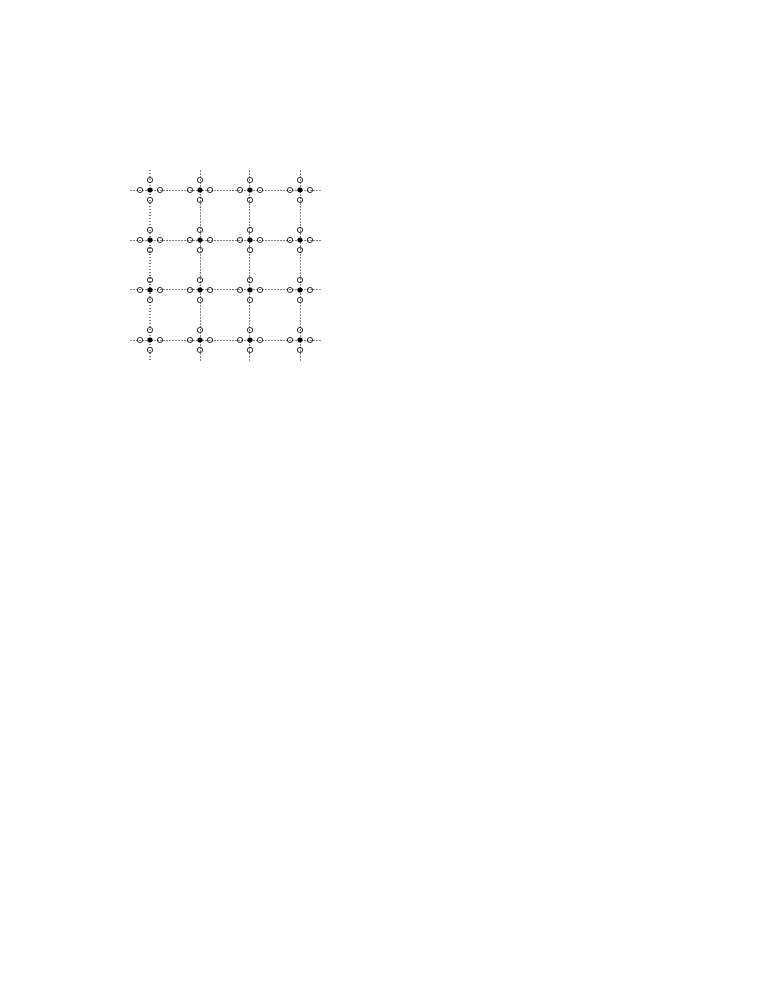
\includegraphics[width=0.5\textwidth]{graphics/main_aux_grids}
\end{center}
\caption{Illustration of main grid (filled circles) and auxiliary grid (empty circles) used to compute the Cauchy-Green strain. The variable \lstinline!auxGridRelDelta! specifies the grid spacing of the auxiliary grid relative to the main grid spacing.}
\label{f:main and auxiliary grids}
\end{figure}

The function \lstinline!eig_cgStrain! provides the option to calculate eigenvectors from the auxiliary grid, but eigenvalues from the main grid. We have found that for flows defined analytically the eigenvalues should be calculated from the main grid whereas for the flows defined by datasets, using the auxiliary grid gives better results.

As stated, typically we set the main grid resolution of the Cauchy-Green strain tensor to around 500 grid points. For a square domain, this implies the velocity equations must be integrated, after including 4 auxiliary grid points around every main grid point, at 1.25 million grid points. The natural way to perform these integration calculations would be to solve a two dimensional first-order ODE system at every grid point and iterate over every grid point in a for-loop. With 1.25 million grid points this calculation can take an excessively long time. To alleviate this problem, we solve the flow equations in a vector form where the equations at all grid points are combined into a single system of equations, even though the system is composed of independent blocks of two dimensional first-order ODE systems. MATLAB's \lstinline!ode45! function is used to perform the integration and the flow integration typically takes five to ten minutes with default error tolerances. The drawback of vector form integration is that memory requirements can become excessive at high resolutions. Furthermore, writing the velocity function in vector form is more error-prone than the simpler two dimensional form.

The Cauchy-Green strain tensor can have singularities, i.e., $C_{t_0}^t(\boldsymbol x_0) = I$. Such points are isolated in general\parencite{delmarcelle94}, therefore no special accommodations are made in computations for singularities of the Cauchy-Green strain tensor.

\subsubsection{Special case: incompressible velocity fields}

Flows that are incompressible, meaning $D \cdot \boldsymbol v = 0$, satisfy the relation $\lambda_1(\boldsymbol x_0) \lambda_2(\boldsymbol x_0) = 1, \forall \: \boldsymbol x_0 \: \in \: U$\parencite{arnold78:_mathem}. This gives the possibility of imposing incompressibility when calculating the eigenvalues of the Cauchy-Green strain tensor by first calculating $\lambda_2$ and then setting $\lambda_1(\boldsymbol x_0) = 1/\lambda_2(\boldsymbol x_0)$. This procedure should be applied carefully since by changing $\lambda_1$ but not $\boldsymbol \xi_1$, the error in satisfying the eigenvalue equation for the Cauchy-Green strain tensor may increase.

At some grid points it may occur that $\lambda_2 < 1$ due to numerical integration errors of the flow velocity equations. By setting integration tolerances to smaller values the number of grid points with $\lambda_2 < 1$ can be reduced. Nonetheless, some grid points can be so close to singularities of the Cauchy-Green strain tensor that satisfying $\lambda_2 \geq 1$ everywhere could be excessively computationally costly. Therefore the function \lstinline!eig_cgStrain! records the number of points at which incompressibility cannot be imposed and this measure can guide setting appropriate integration tolerances.

\subsubsection{Special case: data-defined velocity fields}

Velocity fields defined by datasets require pre-processing prior to performing the integration that yields the flow map. An interpolation function must be written to enable evaluating the velocity function at arbitrary points in $U$ and at arbitrary times between $t_-$ and $t_+$. MATLAB's interpolation functions can be used in the velocity function. In section \ref{sec:oceandataset} we present an example for LCSs computed for an ocean dataset and details of the interpolation function are given.

Beyond the pre-processing needed to obtain the Cauchy-Green strain tensor eigenvalues and eigenvectors, no special manipulations are needed to treat data-defined flow. It may be however, that parameter values giving good results with analytically defined flows need adjustment prior to processing data-defined velocity fields.

\subsection{Shear LCS}

Shear LCSs, or coherent Lagrangian vortices, are closed orbits in the Lagrangian shear vector fields $\boldsymbol \eta_{\pm}$ defined in Equation~\eqref{eq:etafields}. We find closed orbits by integrating lambda-lines starting from a Poincare section and evaluating the return map. A lambda-line returning to its starting point is a shear LCS. The main steps of the algorithm used to calculate shear LCS are enumerated in Table~\ref{t:Shear LCS algorithm} and described in detail below. The syntax of shear LCS functions in LCS Tool is in Table~\ref{t:Shear LCS functions}.

\begin{table}
\begin{center}
\begin{enumerate}
\item Position Poincare sections in flow domain to specify initial positions of lambda-lines
\item Integrate lambda-lines tangent to $\boldsymbol \eta_{\pm}$ (see Equation~\eqref{eq:etafields}.)
\item Calculate Poincare return map
\item Find closed orbits positions from Poincare return map
\item Identify outermost closed orbit
\end{enumerate}
\end{center}
\caption{Algorithm to calculate Shear LCS}
\label{t:Shear LCS algorithm}
\end{table}

\begin{table}
\begin{tabular}{|c|p{.7\textwidth}|}
\hline \hline
\multicolumn{2}{|p{\textwidth}|}{\lstinline![shearline.etaPos,shearline.etaNeg] = lambda_line(cgEigenvector,cgEigenvalue,lambda)!}\\
\hline
\lstinline!cgEigenvector! & array of Cauchy-Green strain eigenvectors\\
\hline
\lstinline!cgEigenvalue! & array of Cauchy-Green strain eigenvalues\\
\hline
\lstinline!lambda! & scalar lambda value in Equation~\eqref{eq:eta}\\
\hline \hline
\multicolumn{2}{|p{\textwidth}|}{\lstinline![closedOrbits,orbits] = poincare_closed_orbit_multi(domain,resolution,shearline,PSList)!}\\
\hline
\lstinline!domain! & array to define flow domain\\
\hline
\lstinline!resolution! & $1 \times 2$ array to define Cauchy-Green strain main grid resolution\\
\hline
\lstinline!shearline! & structure of arrays of $\eta_+$ and $\eta_-$ values on main grid\\
\hline
\lstinline!PSList! & structure for Poincare section end-points, number of lambda-lines launched from Poincare section, and maximum closed lambda-line length\\
\hline
\lstinline!nBisection! & optional number of bisection steps to refine zero crossings of Poincare return map. Default is 5.\\
\hline
\lstinline!dThresh! & optional threshold to discard discontinuous zero crossings of Poincare return map. Default is $10^{-2}$.\\
\hline
\lstinline!odeSolverOptions! & optional \lstinline!odeset! structure to specify lambda-line integration parameters\\
\hline
\lstinline!periodicBc! & optional $1 \times 2$ logical array to specify periodic boundary conditions. Default is \lstinline![false,false]!.\\
\hline \hline
\end{tabular}
\caption{LCS Tool shear LCS functions syntax}
\label{t:Shear LCS functions}
\end{table}

The first step is to set the position of Poincare sections as straight lines in regions where closed lambda-lines are expected. The Poincare section must be oriented such that the first endpoint is close to the center of the expected eddy and the second endpoint is outside the expected eddy. There is no definite procedure for deciding the position of Poincare sections. Possibilities include an examination of the finite time Lyapunov exponent field of the flow, or some prior knowledge of where coherent eddies are be expected. Additionally, the number of lambda-lines launched from the Poincare section, \lstinline!poincareSection.numPoints!, must be defined. A good default is 100.

The second step is to integrate the lambda-lines to obtain the Poincare return map. Integration of lambda-lines is performed with the $\boldsymbol \eta_+$ and $\boldsymbol \eta_-$ vector fields defined on the main grid. These vector fields are derived from eigenvalues and eigenvectors as described in~\textcite{farazmand12:_comput_lagran}. The eigenvector fields have orientation discontinuities, therefore the vector field must be locally reoriented for the integration. The algorithm used to perform variable step-size integration in vector fields with orientation discontinuities is enumerated in Table~\ref{t:variable step integration} and illustrated in Figure~\ref{f:variable step integration}. Linear interpolation is used when interpolating $\boldsymbol \eta_\pm$ within a grid element, since using higher order interpolation would necessitate verifying that there are no orientation discontinuities at more than only the four nearest grid points. Detection of orientation discontinuities is achieved by checking the inner product of the vector fields at adjacent grid points. Then, rotations exceeding 90\degree\, are classified as orientation discontinuities and are corrected before linear interpolation. Thus when setting the Cauchy-Green strain tensor main grid resolution, a histogram of eigenvector field rotations may be calculated to ensure all rotations are well below 90\degree\, or almost 180\degree.

\begin{table}
\begin{enumerate}
\item Linearly interpolate vector field orientation at initial position
\item At next position, check whether vector field has rotated by over 90\degree, if yes, flip the vector field orientation by 180\degree.
\item Stop integration when lambda-line returns to Poincare section, lambda-line reaches the domain boundary, or maximum integration length has been reached.
\end{enumerate}
\caption{Algorithm used for variable time step integration of lambda-lines.}
\label{t:variable step integration}
\end{table}

\begin{figure}
\begin{center}
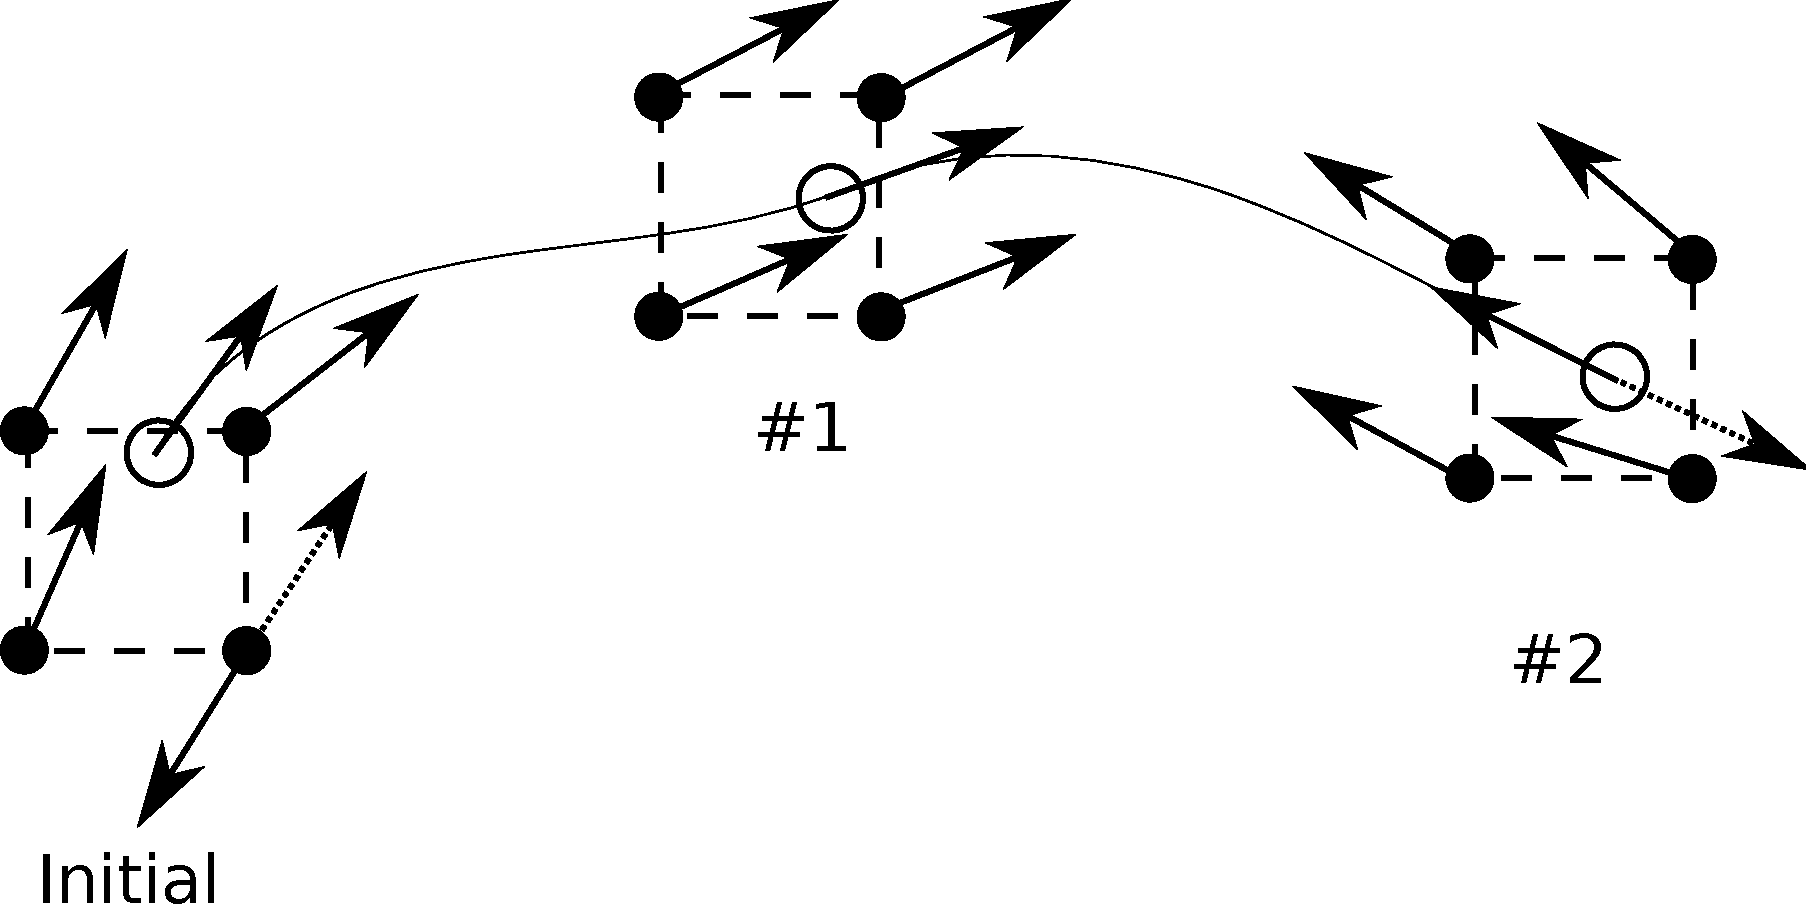
\includegraphics[width=0.8\textwidth]{graphics/variable_step_integration}
\end{center}
\caption{Schematic illustration of lambda-line variable time step integration. At the initial point, there is an orientation discontinuity at the lower right grid point that must be corrected prior to linear interpolation. At point \#1, no orientation discontinuities are present. At point \#2 the interpolated $\eta_\pm$ vector must be rotated by 180\degree\,to match the orientation of the trajectory.}
\label{f:variable step integration}
\end{figure}

An example of a Poincare return map produced from integration of the $\boldsymbol \eta_\pm$ field is shown in Figure~\ref{f:Poincare return map}. Well behaved orbits will return to the Poincare section and their integration will be stopped using ODE event detection. Some orbits may however deviate far from the Poincare section and their integration could take inordinately long. To limit this behavior, a maximum orbit length, \lstinline!poincareSection.orbitMaxLength!, is specified. In practice, viewing the Poincare section as the radius of a circle and setting the maximum lambda-line integration length to twice the circumference gives good results. In Figure~\ref{f:Poincare return map}, circle markers indicate closed orbit positions. Closed orbits exist where the Poincare return map, the distance between the final and the initial point of the orbit $P(s)-s$, is zero. The function \lstinline!poincare_closed_orbit_multi! performs the computations. In Figure~\ref{f:Poincare return map} not all zero crossings have circles. This is because a threshold parameter \lstinline!dThresh! is used to discard those zero crossings that appear in regions with high numerical noise. Its default value is 1\% of the length of the Poincare section. The position of each detected zero crossing is refined by iteratively bisecting the interval of the zero crossing. If after a predetermined number of iterations, \lstinline!nBisection! whose default value is five, the two points around the zero crossing have absolute values above \lstinline!dThresh!, the zero crossing is discarded. Once all valid closed lambda-line orbits have been located, the outermost orbit of every Poincare section is identified as a shear LCS.

\begin{figure}
\begin{center}
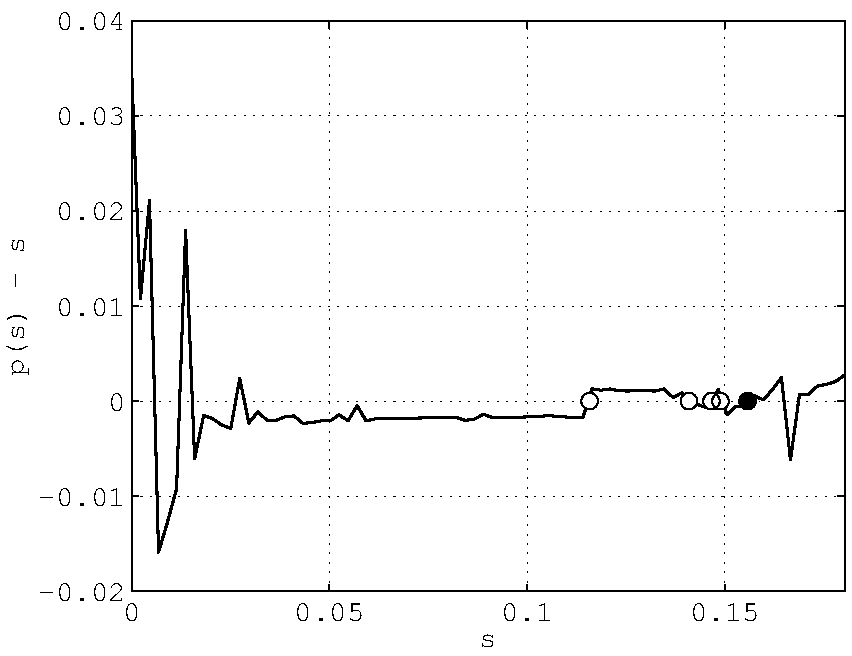
\includegraphics[width=0.8\textwidth]{graphics/double_gyre/poincare_return_map}
\end{center}
\caption{Example of a Poincare return map obtained for shear LCS. Circle markers indicate closed orbit positions. The filled circle indicates the outermost closed orbit and shear LCS.}
\label{f:Poincare return map}
\end{figure}

\subsection{Hyperbolic LCS}

The main steps of the algorithm used to calculate hyperbolic LCSs are enumerated in Table~\ref{t:Hyperbolic LCS algorithm}. The main function to compute hyperbolic LCS in LCS Tool is \lstinline!seed_curves_from_lambda_max! and its syntax is given in Table~\ref{t:seed_curves_from_lambda_max syntax}.

\begin{table}
\begin{enumerate}
\item Define a local maximization distance.
\item Find all local maxima of $\lambda_2$ on the main grid such that they are maxima within a circle with a radius equal to the local minimization distance.
\item Define a maximum strainline length
\item Integrate a strainline forward and backward according to Equation~\eqref{eq:strainline} and using the largest $\lambda_2$ local maximum as the initial position. Integrate until the strainline has attained the maximum strainline length, or until it has reached the domain boundary.
\item Flag any remaining local maxima of $\lambda_2$ within the minimization distance of the strainline as ineligible initial positions for subsequent strainlines
\item Continue integrating strainlines using local maxima of $\lambda_2$ as initial positions until no eligible local maxima of $\lambda_2$ remain.
\end{enumerate}
\caption{Algorithm to calculate strainline hyperbolic LCSs. Algorithm for stretchline hyperbolic LCSs is similar.}
\label{t:Hyperbolic LCS algorithm}
\end{table}

\begin{table}
\begin{center}
\begin{tabular}{|c|p{.7\textwidth}|}
\hline \hline
\multicolumn{2}{|p{\textwidth}|}{\lstinline![curvePosition,curveInitialPosition] = seed_curves_from_lambda_max(distance,cgEigenvalue,cgEigenvector,flowDomain,flowResolution)!}\\
\hline
\lstinline!distance! & threshold distance for placement of lambda maxima\\
\hline
\lstinline!cgEigenvalue! & array of Cauchy-Green strain eigenvalues\\
\hline
\lstinline!cgEigenvector! & array of Cauchy-Green strain eigenvectors\\
\hline
\lstinline!flowDomain! & $2 \times 2$ array to define flow domain\\
\hline
\lstinline!flowResolution! & $1 \times 2$ array to define Cauchy-Green strain main grid resolution\\
\hline
\lstinline!periodicBc! & optional $1 \times 2$ logical array to specify periodic boundary conditions. Default is \lstinline![false,false]!.\\
\hline
\lstinline!nMaxCurves! & optional maximum number of curves (i.e. strainlines of stretchlines) to generate. Default is \lstinline!numel(cgEigenvalue)!.\\
\hline
\lstinline!odeSolverOptions! & optional \lstinline!odeset! structure to specify flow map integration parameters\\
\hline \hline
\end{tabular}
\end{center}
\caption{Syntax of the function \lstinline!seed_curves_from_lambda_max!}
\label{t:seed_curves_from_lambda_max syntax}
\end{table}

Strainlines, trajectories of the $\boldsymbol \xi_1$ vector field, are integrated starting from local maxima of $\lambda_2$ on the main grid. The local maximization distance \lstinline!distance! is defined. This distance is set to a value between two and five grid points, since it represents the number of grid points over which the Cauchy-Green strain tensor is susceptible to numerical noise from integration. Thus, the local maximization distance is expected to be a function of variable time step integration tolerances. A record is made of all grid points where $\lambda_2$ is maximal within a circle whose radius equals the defined maximization distance. Then the first strainline is integrated from the largest of all the local maxima in both directions, i.e., integrating $\boldsymbol \xi_1$ and $-\boldsymbol \xi_1$. Similarly to lambda-lines, this integration must take into account eigenvector field orientation discontinuities. Prior to initiating strainline integration, a maximum length is defined. Strainlines are then integrated until reaching the domain boundary or the maximum length. The maximum length may be seen as safety factor to prevent highly sinuous strainlines leading to inordinately long computations; the maximum length should be set such that most strainlines stop at the domain boundary. Once a strainline position has been calculated, local maxima of $\lambda_2$ within the minimization distance are flagged as ineligible initial positions for subsequent strainlines. After the first strainline has been obtained and any ineligible local maxima of $\lambda_2$ have been flagged, the next strainline is integrated starting form the highest eligible maximum of $\lambda_2$. The process continues until all eligible local maxima of $\lambda_2$ have been used to initialize strainline integration. These calculations are performed by the function \lstinline!seed_curves_from_lambda_max!. Note that once a strainline integration has begun, it may progress so as to be within the local minimization distance of an existing strainline. In other words, the local minimization distance controls where strainlines begin, but not where they stop.

A further point important to note is the existence of hyperbolic LCS inside elliptic LCS. This may seem contradictory when accustomed to LCSs not crossing, however, numerical experimentation with LCS calculations overlaid with color tracer advection reveals that hyperbolic LCS can cross elliptic barriers and have an impact on the tracer pattern inside elliptic regions. At crossing points a line segment of an elliptic LCS, oriented along $\boldsymbol \eta_\lambda^{\pm}$, does not stretch, while a segment of a strainline, oriented along $\boldsymbol \xi_1$, repels fluid normally at a maximal rate and shrinks at a maximal rate. Figure~\ref{fig:ocean_dataset_colortracer} illustrates the effect of strainlines on tracer particles inside elliptic regions. Color-coded final positions show large gradients along strainlines, directly showing that particles are strongly repelled by the LCS and therefore end in different positions.

\begin{figure}[hbt]
\centering
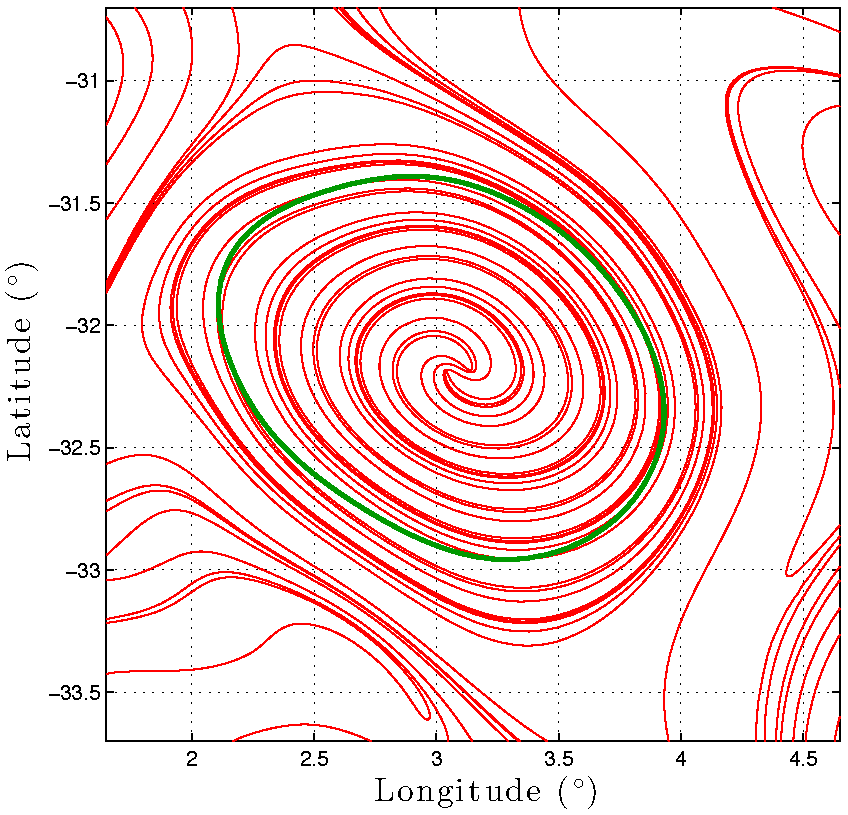
\includegraphics[width=0.49\textwidth]{graphics/ocean_dataset/LCS_fwd_coherent_eddy}
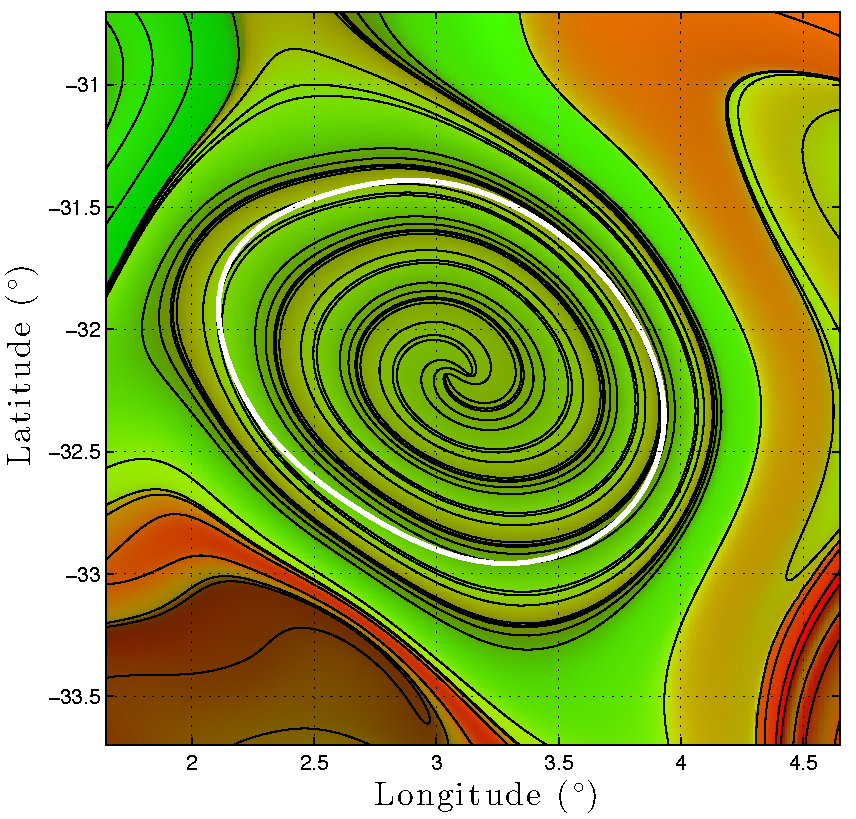
\includegraphics[width=0.49\textwidth]{graphics/ocean_dataset/LCS_fwd_colortracer}
\caption{(Left) Elliptic LCS (green) with hyperbolic normally repelling LCS (red) inside. (Right) Final positions $\boldsymbol x_t = F_{t_0}^t(\boldsymbol x_0)$ of tracer particles are plotted with the x-position encoded in red and y-position encoded in green color. The impact of the repulsive property of hyperbolic LCS on the tracer particles can not only be observed outside, but also inside the elliptic region. Hyperbolic LCS mark lines of high color gradients, corresponding to tracer particles that start on both sides of the LCS, are repelled, and end up in distinct locations.}
\label{fig:ocean_dataset_colortracer}
\end{figure}

\clearpage

\section{Examples}
In this section we present examples showing how to use LCS Tool to obtain LCSs in different flows, namely a double gyre, a jet, and an oceanic geostrophic flow. All three examples are available as demonstration files in the demo folder of LCS Tool. By executing these scripts, readers can follow LCS Tool computations step-wise.

\subsection{The double gyre}
The double gyre is a model for a time-dependent two gyre system observed in geophysical flows \parencite{shadden05:_defin_lagran_lyapun}. It consists of two counter rotating sinusoidal vortices with a harmonically oscillating line in-between. The velocity equations are:
\begin{equation}
\begin{split}
\dot x = -\pi A \sin[\pi f(x,t)] \cos(\pi y)\\
\dot y = \pi A \cos[\pi f(x,t)] \sin(\pi y) \frac{\partial f(x,t)}{\partial x}\\
f(x,t) = \epsilon \sin(\omega t) x^2 + [1 - 2 \epsilon \sin(\omega t)] x.
\end{split}
\label{eq:double gyre derivative equations}
\end{equation}
The MATLAB function corresponding to these equations is given in Listing~\ref{l:double gyre derivative} and shows how to specify a derivative function that supports vector form integration.

\begin{lstlisting}[caption={Double gyre derivative function corresponding to Equations~\eqref{eq:double gyre derivative equations}.},label=l:double gyre derivative]
function derivative_ = derivative(t,x,epsilon,amplitude,omega)

idx1 = 1:2:numel(x)-1;
idx2 = 2:2:numel(x);

a = epsilon*sin(omega*t);
b = 1 - 2*epsilon*sin(omega*t);
forcing = a*x(idx1).^2 + b*x(idx1);

derivative_ = nan(size(x));

derivative_(idx1) = -pi*amplitude*sin(pi*forcing).*cos(pi*x(idx2));
derivative_(idx2) = pi*amplitude*cos(pi*forcing).*sin(pi*x(idx2)).*(2*a*x(idx1) + b);
\end{lstlisting}

In what follows, the parameter values are: $A = 0.1$, $\epsilon = 0.1$, $\omega = \pi/5$. The flow timespan is $t \in [0,5]$ and the domain is $x \in [0,2]$, $y \in [0,1]$.

By examining the FTLE, we can position Poincare sections to detect lambda-line LCSs. An LCS Tool script to perform this operation is given in Listing~\ref{l:double gyre lambda-line LCS} where two Poincare sections are defined. In the script we have set error tolerances for integration of the Cauchy-Green strain tensor and lambda lines. These numerical parameters help achieve convergence.

\lstinputlisting[caption={Double gyre script for lambda-line LCSs},label=l:double gyre lambda-line LCS]{listings/double_gyre/lambda_lcs.m}

In Figure~\ref{fig:double_gyre_lambda_lcs_convergence} the resolution of the  Cauchy-Green strain tensor is varied from $500 \times 250$ to $1000 \times 500$. The location of the outermost closed lambda-line changes little, demonstrating convergence.

\begin{figure}[hbt]
  \centering
  \includegraphics[width=.8\textwidth]{graphics/double_gyre/lambda_lcs_convergence_500}
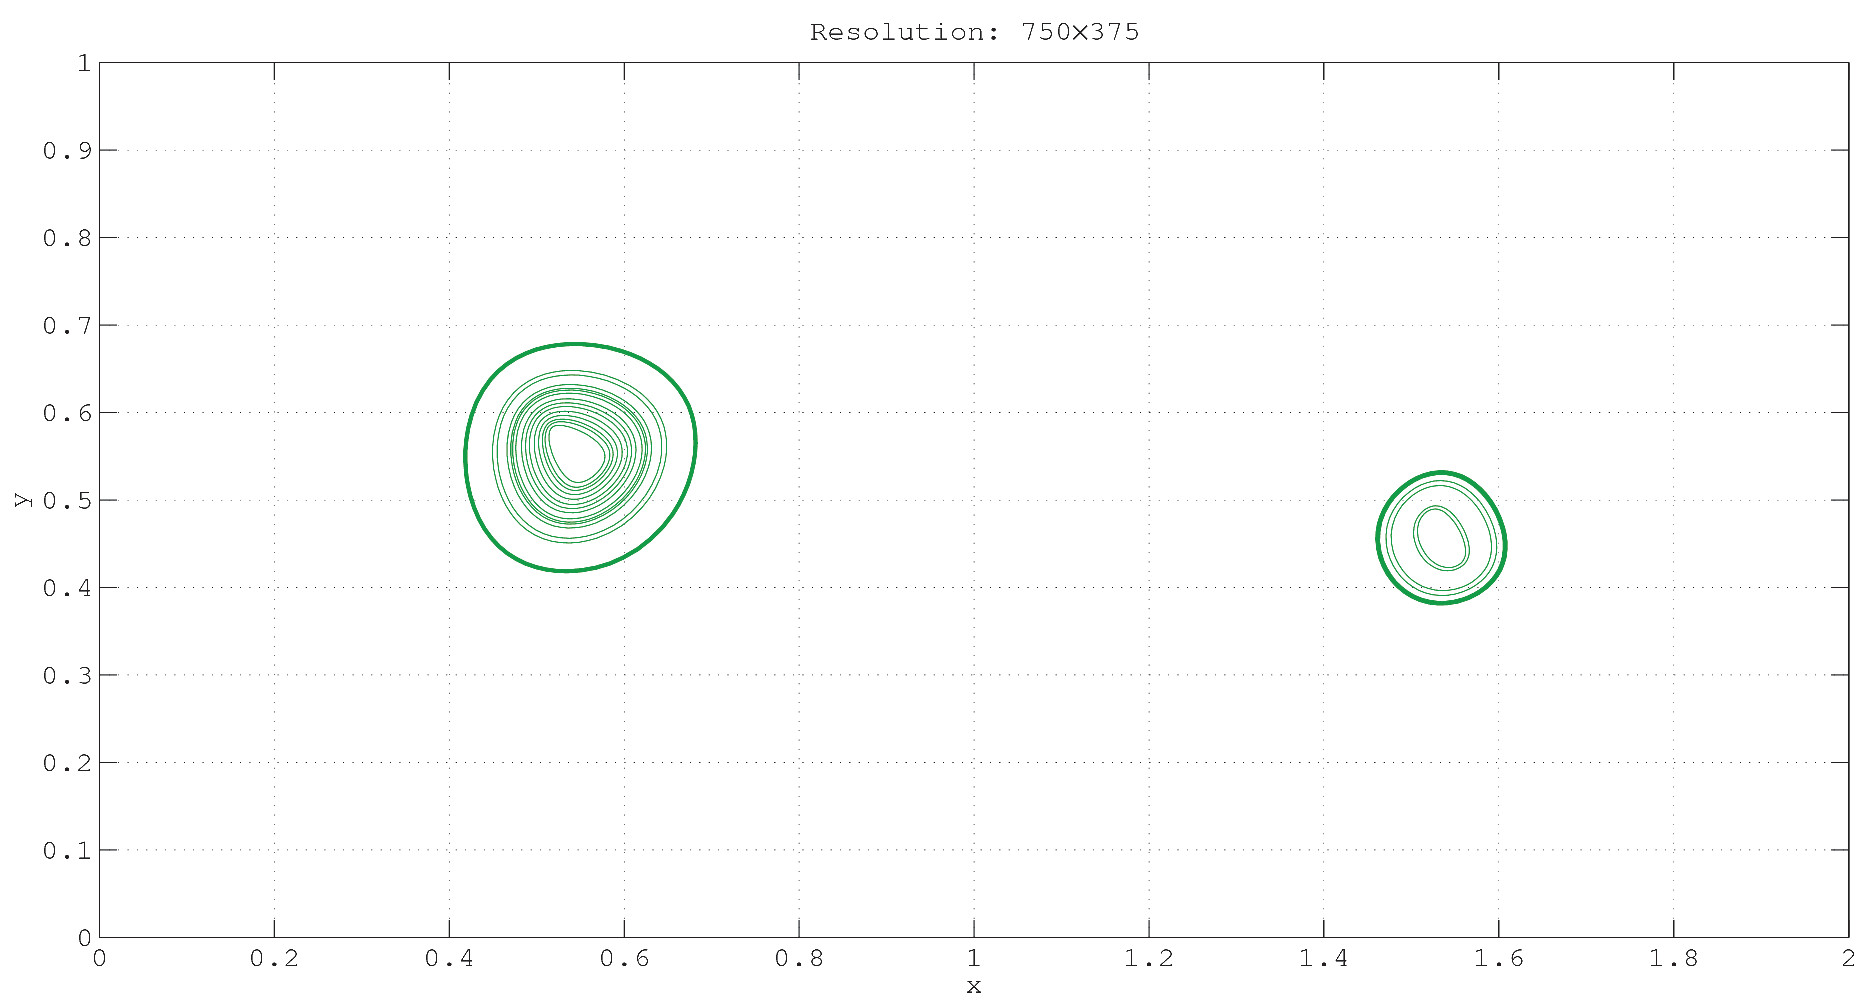
\includegraphics[width=.8\textwidth]{graphics/double_gyre/lambda_lcs_convergence_750}
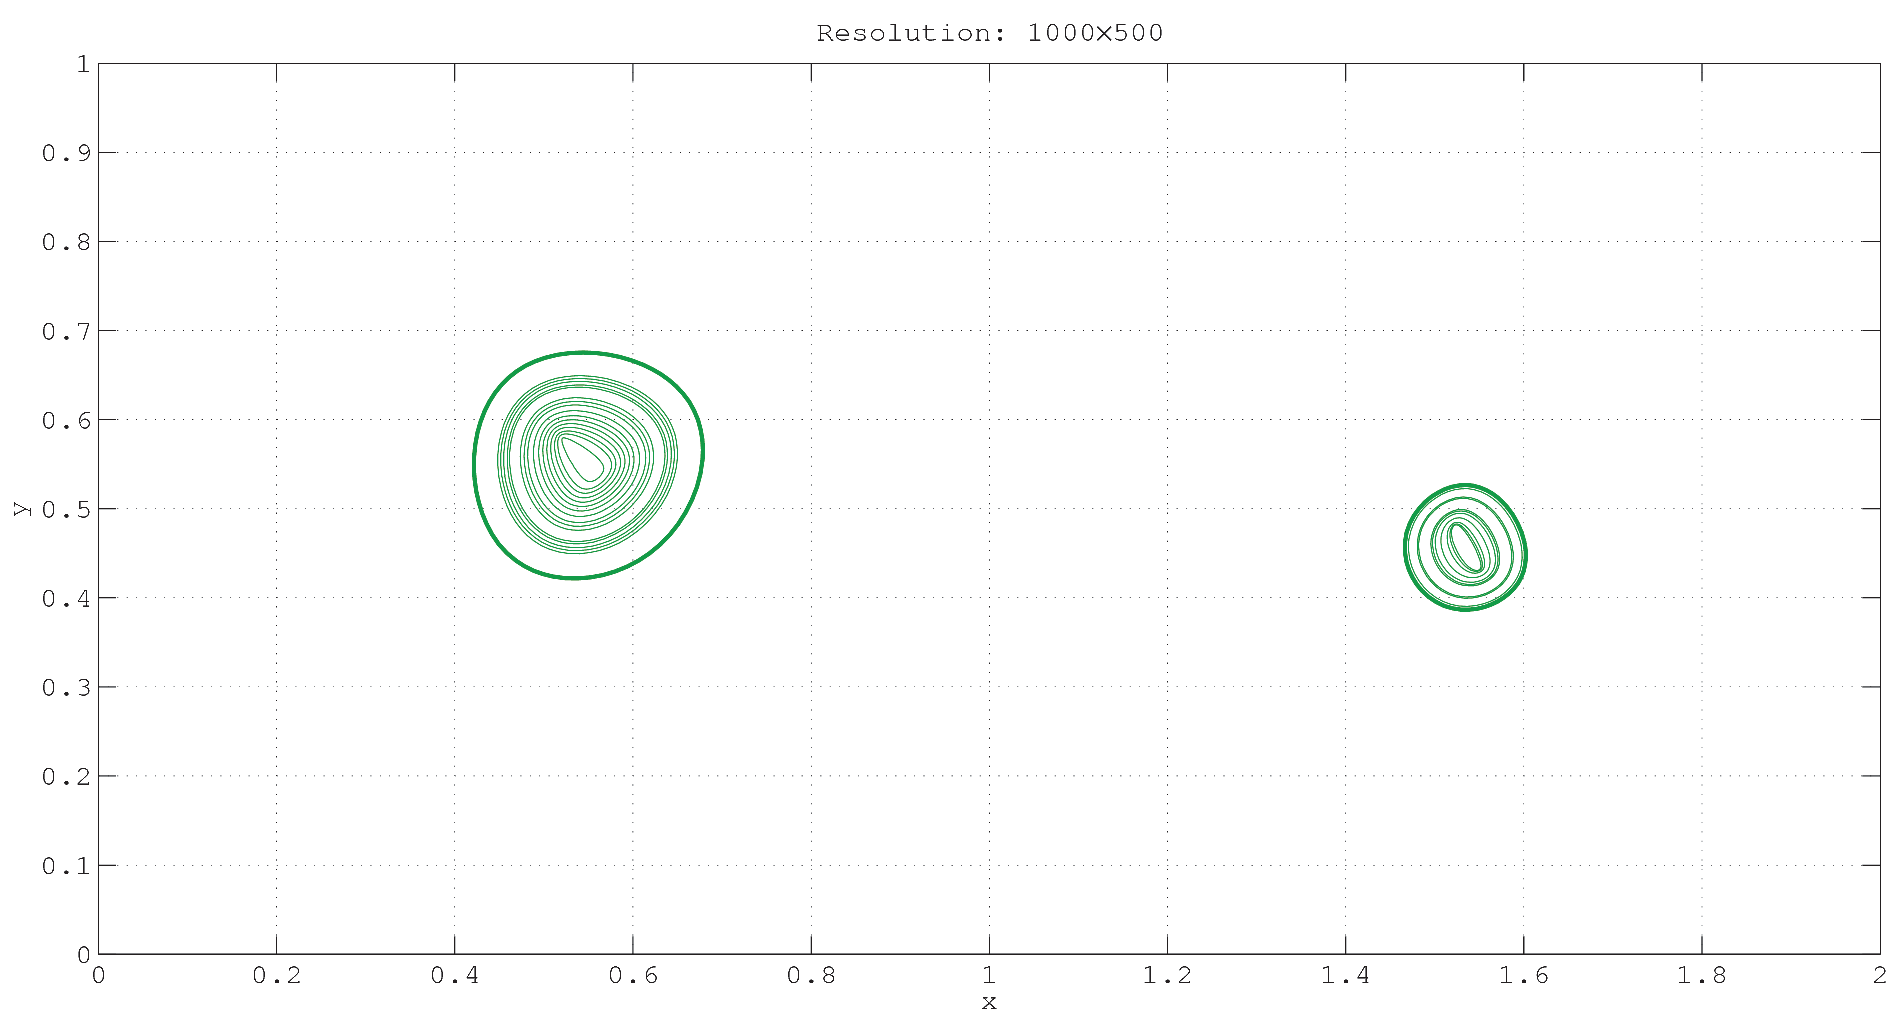
\includegraphics[width=.8\textwidth]{graphics/double_gyre/lambda_lcs_convergence_1000}
  \caption{Double gyre closed lambda-lines at varying resolutions with FTLE background}
  \label{fig:double_gyre_lambda_lcs_convergence}
\end{figure}

We continue the example by adding the calculation of hyperbolic strainline and stretchline LCSs. Figures~\ref{fig:double_gyre_lambda_strain_lcs} and~\ref{fig:double_gyre_lambda_stretch_lcs} show the results and Listing~\ref{lst:double_gyre_lambda_strain_stretch_lcs} gives the LCS Tool commands. The local maximization distance is set larger for stretchlines than for strainlines usually. This is because strainlines follow ridges of $\lambda_2$ maxima whereas stretchlines do not follow ridges of $\lambda_1$ minima.

\begin{figure}
  \centering
  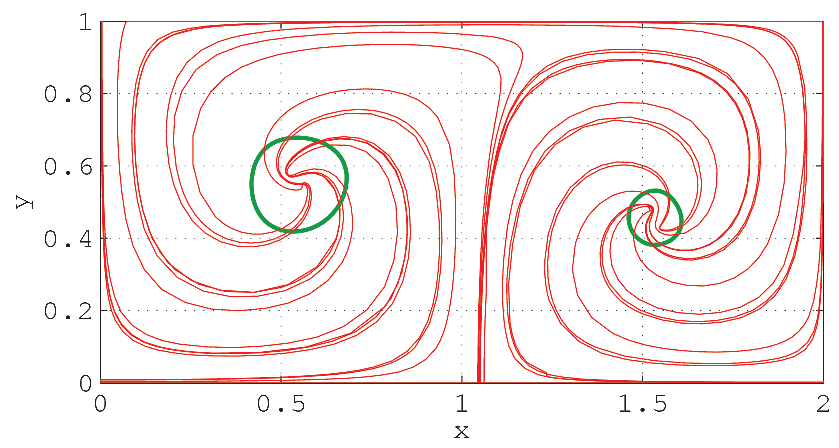
\includegraphics[width=\textwidth]{graphics/double_gyre/lambda_strain_lcs}
  \caption{Double gyre lambda-line and strainline LCSs}
  \label{fig:double_gyre_lambda_strain_lcs}
\end{figure}

\begin{figure}
  \centering
  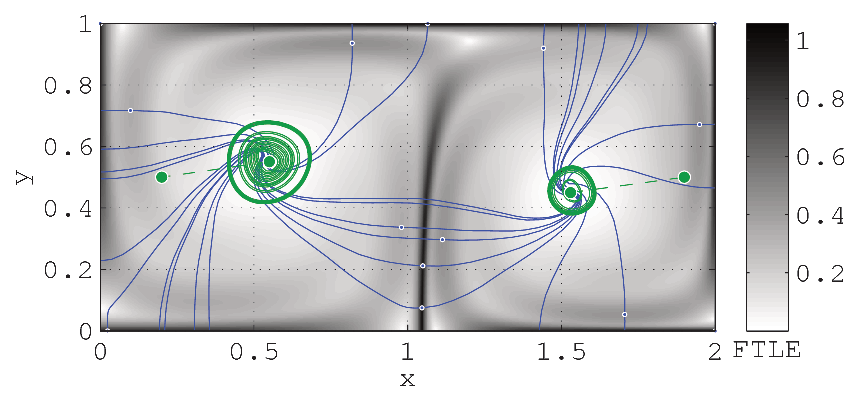
\includegraphics[width=\textwidth]{graphics/double_gyre/lambda_stretch_lcs}
  \caption{Double gyre lambda-line and stretchline LCSs}
  \label{fig:double_gyre_lambda_stretch_lcs}
\end{figure}

\lstinputlisting[caption={LCS Tool commands for double gyre strainline and stretchline LCSs. Condensed version of the LCS Tool script \lstinline!demo/double_gyre/hyperbolic_shear_lcs.m! },label=lst:double_gyre_lambda_strain_stretch_lcs]{listings/double_gyre/lambda_strain_stretch_lcs.m}

\clearpage

\subsection{Bickley jet}

The Bickley jet models a meandering zonal jet flanked above and below by
counter rotating vortices. This is an idealized model of geophysical flows
such as the polar night jet perturbed by a Rossby
wave\parencite{haller12:_geodes_theor_trans_barrier_two_dimen_flows,beron-vera10:_invar_lagran}.

The velocity is given by $\boldsymbol{v}(x,y,t) = (-\partial_y \psi, \partial_x \psi)$ where
\begin{gather*}
\psi(x,y,t) = \psi_0(x,y) + \psi_1(x,y,t),\\
\psi_0(x,y) = c_3 y - U L_y \tanh\frac{y}{L_y} + \epsilon_3 U L_y \mathrm{sech}^2\frac{y}{L_y} \cos k_3 x,\\
\psi_1(x,y,t) = U L_y \mathrm{sech}^2\frac{y}{L_y} \mathrm{Re}\left[ \sum_{n=1}^2 \epsilon_n f_n(t) e^{i k_n x}\right].
\end{gather*}
As a forcing function we choose a chaotic solution of the Duffing oscillator, specifically
\begin{gather*}
\frac{d \phi_1}{dt} = \phi_2,\\
\frac{d \phi_1}{dt} = -0.1 \phi_2 - \phi_1^3 + 11 \cos(t),\\
f_{1,2}(t) = 2.625 \times 10^{-2} \phi_1(t/6.238 \times 10^5)
\end{gather*}
The parameter values we use are: $U = 62.66$, $c_2 = 0.205 U$, $c_3 = 0.461 U$, $L_y = 1.77 \times 10^6$, $\epsilon_1 = 0.0075$, $\epsilon_2 = 0.04$, $\epsilon_3 = 0.3$, $L_x = 6.371 \times 10^6 \pi$, $k_n = 2 n \pi/L_x$, $\sigma_1 = 0.5 k_2 (c_2 - c_3)$, $\sigma_2 = 2 \sigma_1$.

Figure~\ref{fig:Bickley_jet_lambda_LCS_full} shows lambda-line LCS of the Bickley jet with the FTLE in the background. The figure demonstrates a poor result since the LCSs change shape significantly between eddies. To address this problem we could adjust numerical parameters such as the resolution, but instead we will analyze lambda-line closed orbits of one vortex for a short timespan.

\begin{figure}
  \centering
  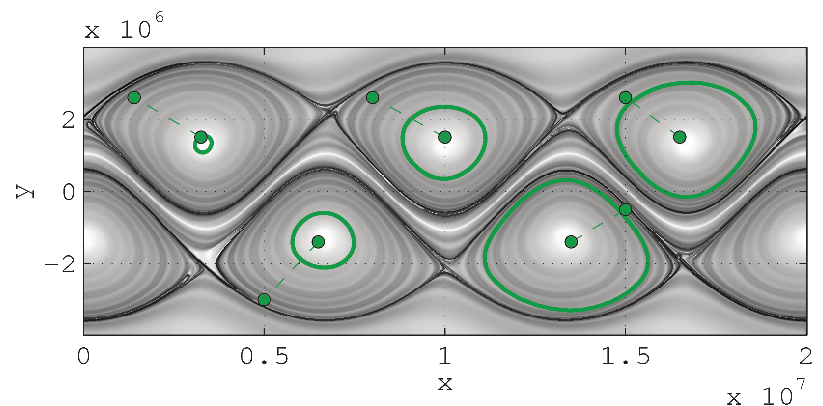
\includegraphics[width=.85\textwidth]{graphics/bickley_jet/lambda_lcs_full}
  \caption{Bickley jet lambda-line LCSs}
  \label{fig:Bickley_jet_lambda_LCS_full}
\end{figure}

Figure ~\ref{fig:Bickley jet lambda lcs convergence} shows convergence of the lambda-line elliptic LCSs. The LCS Tool script used to produce that figure are based on the script \lstinline!demo/bickley_jet/hyperbolic_shear_lcs.m! which is given in  Listing~\ref{lst:Bickley jet hyperbolic_shear_lcs subset}. It is worth pointing out that in order to obtain closed orbits, $\lambda = 0.995$; with $\lambda = 1$ no closed orbits exist.

\lstinputlisting[caption={Bickley jet script for hyperbolic and shear LCSs. Subset of \lstinline!demo/bickley_jet/hyperbolic_shear_lcs.m!},label=lst:Bickley jet hyperbolic_shear_lcs subset]{listings/bickley_jet/hyperbolic_shear_lcs_subset.m}

\begin{figure}[hbt]
  \centering
  \includegraphics[width=.7\textwidth]{graphics/bickley_jet/lambda_lcs_convergence_400}
\includegraphics[width=.7\textwidth]{graphics/bickley_jet/lambda_lcs_convergence_500}
\includegraphics[width=.7\textwidth]{graphics/bickley_jet/lambda_lcs_convergence_600}
  \caption{Bickley jet closed lambda-line at varying resolutions}
  \label{fig:Bickley jet lambda lcs convergence}
\end{figure}

Strainline LCSs are shown in Figure~\ref{fig:Bickley_jet_strain_lcs} and stretchline LCSs are shown in Figure~\ref{fig:Bickley_jet_stretch_lcs}.

\begin{figure}
  \centering
  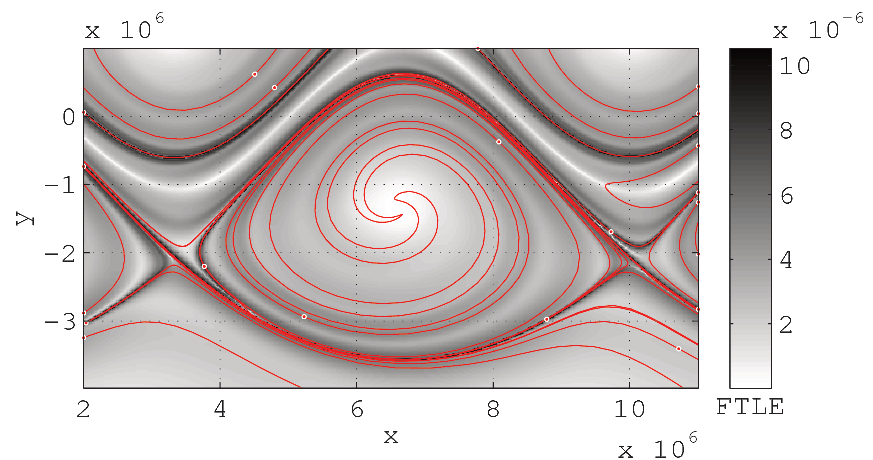
\includegraphics[width=.85\textwidth]{graphics/bickley_jet/strain_lcs}
  \caption{Bickley jet strainline LCSs}
  \label{fig:Bickley_jet_strain_lcs}
\end{figure}

\begin{figure}
  \centering
  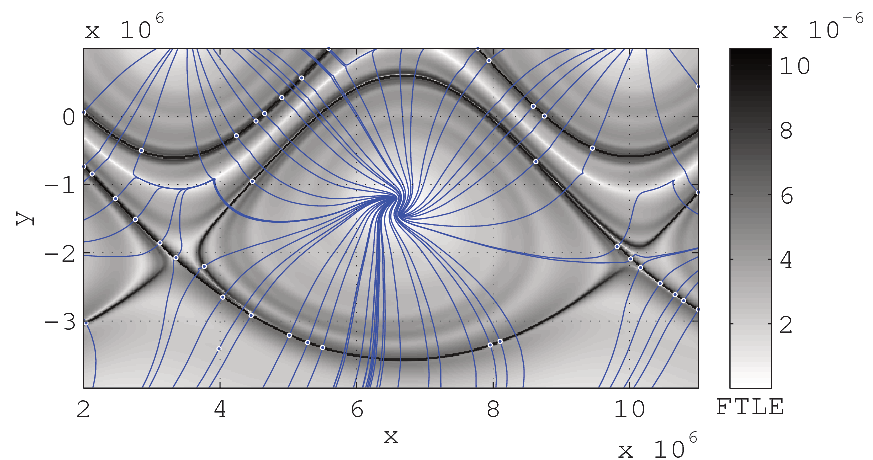
\includegraphics[width=.85\textwidth]{graphics/bickley_jet/stretch_lcs}
  \caption{Bickley jet stretchline LCSs}
  \label{fig:Bickley_jet_stretch_lcs}
\end{figure}

\clearpage

\subsection{Ocean dataset}
\label{sec:oceandataset}

For the last example, corresponding to the ocean dataset demo files in LCS Tool, we choose a measured geophysical flow. In contrast to the previous analytic examples, the two dimensional incompressible velocity field is presented as a dataset with discrete temporal and spatial resolution. Our region of interest is a small domain in the South Atlantic Ocean, where exceptionally coherent eddies, Agulhas rings, were recently found using methods provided by LCS Tool \parencite{haller13:_coher_lagran}. The oceanic velocity field is obtained from altimetric satellite measurements of the sea surface height under the assumption that the flow is geostrophic. Under this assumption the sea surface height $\eta$ serves as a stream-function and in a longitude-latitude $(\varphi,\theta)$ coordinate system the evolution of a fluid particle is given by
\begin{eqnarray}
\dot{\varphi}(\varphi,\theta,t) = -\frac{g}{R^2 f(\theta) \cos\theta}\partial_{\theta}\eta(\varphi,\theta,t)\label{eq:dtlon}\\
\dot{\theta}(\varphi,\theta,t) = +\frac{g}{R^2 f(\theta) \cos\theta}\partial_{\varphi}\eta(\varphi,\theta,t)
\label{eq:dtlat}
\end{eqnarray}
where $g$ is the gravitational acceleration, $R$ is the mean radius of Earth, and $f(\theta) \equiv 2\Omega\sin\theta$ is the Coriolis parameter with $\Omega$ being the Earth's mean angular velocity. 

The data is given at a spatial resolution of $1/4\degree$ and a temporal resolution of $7\,\mathrm{days}$. Due to the discrete data, defining the right hand side of Equation~\eqref{eq:dtlon} and~\eqref{eq:dtlat} involves interpolation in space and time with a spline interpolation scheme. An interpolant is generated first, then the function \lstinline!flowdata_derivative! evaluates the interpolants for the zonal and meridional velocity at the needed coordinates. Listing \ref{l:griddedInterp} shows large parts of the code in LCS Tool's ocean demo file \lstinline!hyperbolic_shear_lcs.m!. In lines 8-11 the commands for the interpolation are given.

\begin{lstlisting}[caption={LCS ocean demo: Parts of the demo script included in LCS Tool to compute LCS from an ocean data set},label=l:griddedInterp]
% Input parameters
domain = [0,6;-34,-28];
resolution = [400,400];
timespan = [100,130];

% Velocity definition
...
interpMethod = 'spline';
vlon_interpolant = griddedInterpolant({time,lat,lon},vlon,interpMethod);
vlat_interpolant = griddedInterpolant({time,lat,lon},vlat,interpMethod);
lDerivative = @(t,x,~)flowdata_derivative(t,x,vlon_interpolant,vlat_interpolant);
incompressible = true;

% LCS parameters
% Cauchy-Green strain
cgEigenvalueFromMainGrid = false;
cgAuxGridRelDelta = 0.01;

% Lambda-lines
lambda = 1;
lambdaLineOdeSolverOptions = odeset('relTol',1e-6);

% Strainlines
strainlineMaxLength = 20;
gridSpace = diff(domain(1,:))/(double(resolution(1))-1);
strainlineLocalMaxDistance = 2*gridSpace;
strainlineOdeSolverOptions = odeset('relTol',1e-4);

% Stretchlines
stretchlineMaxLength = 20;
stretchlineLocalMaxDistance = 4*gridSpace;
stretchlineOdeSolverOptions = odeset('relTol',1e-4);
...
% Cauchy-Green strain eigenvalues and eigenvectors
[cgEigenvector,cgEigenvalue] = eig_cgStrain(lDerivative,domain,resolution,timespan,'incompressible',incompressible,'eigenvalueFromMainGrid',cgEigenvalueFromMainGrid,'auxGridRelDelta',cgAuxGridRelDelta);

% Lambda-line LCSs
% Define Poincare sections; ...
poincareSection = struct('endPosition',{},'numPoints',{},'orbitMaxLength',{});
...
poincareSection(1).endPosition = [3.3,-32.1;3.7,-31.6];
poincareSection(2).endPosition = [1.3,-30.9;1.9,-31.1];

% Number of orbit seed points along each Poincare section
[poincareSection.numPoints] = deal(100);

% Set maximum orbit length to twice the expected circumference
nPoincareSection = numel(poincareSection);
for i = 1:nPoincareSection
    rOrbit = hypot(diff(poincareSection(i).endPosition(:,1)),diff(poincareSection(i).endPosition(:,2)));
    poincareSection(i).orbitMaxLength = 2*(2*pi*rOrbit);
end
[shearline.etaPos,shearline.etaNeg] = lambda_line(cgEigenvector,cgEigenvalue,lambda);
closedLambdaLine = poincare_closed_orbit_multi(domain,resolution,shearline,poincareSection,'odeSolverOptions',lambdaLineOdeSolverOptions);
...
% Hyperbolic strainline LCSs
strainlineLcs = seed_curves_from_lambda_max(strainlineLocalMaxDistance,strainlineMaxLength,cgEigenvalue(:,2),cgEigenvector(:,1:2),domain,resolution,'odeSolverOptions',strainlineOdeSolverOptions);
...
stretchlineLcs = seed_curves_from_lambda_max(stretchlineLocalMaxDistance,stretchlineMaxLength,-cgEigenvalue(:,1),cgEigenvector(:,3:4),domain,resolution,'odeSolverOptions',stretchlineOdeSolverOptions);
\end{lstlisting}

For the ocean data, the integration time was chosen to be $T=30$ days (Listing \ref{l:griddedInterp}, line 4), a time larger than the turn over time of the mesoscale eddies in the domain. The resolution of the grid of initial conditions is set to $400\times400$ (line 3) which corresponds to a resolution of roughly 0.015\degree\, and gives good results. With this choice the resolution of the tracer grid is of the order of 15 times higher than the resolution of the velocity field. The flow is integrated and the Cauchy-Green strain tensor is computed by the function \lstinline!eig_cgStrain! (line 35). Incompressibility of the flow is enforced (line 12), the auxiliary grid distance is set to 1\% of the main grid distance (line 17), and eigenvalues are computed from the auxiliary grid (line 16). Lambda-line LCS are computed in line 54, after the Poincare section have been set (line 41-42) and the $\boldsymbol\eta_\pm$ fields have been defined (line 53). Hyperbolic LCS, strainlines and strechlines, are computed in lines 57 and 59, respectively.

Figures~\ref{f:ocean dataset hyperbolic shear lcs details strainline} and \ref{f:ocean dataset hyperbolic shear lcs details stretchline} show elliptic and hyperbolic LCS on 22 November 2006, i.e., the same time instant shown in~\textcite{haller13:_coher_lagran,beron-vera13:_objec_agulh}. Note that here the integration time is $T=30$ days, as opposed to 90 days in their analysis. Since for 90 days the hyperbolic LCSs would be a confusing entanglement of lines, we choose a shorter integration time here, to show hyperbolic LCS together with elliptic LCSs. For the shorter integration time, the analysis with LCS Tool reveals a large coherent eddy bounded by a closed lambda-line at $(3,-32)$ which corresponds to eddy \#2 in Figure~3 of \textcite{beron-vera13:_objec_agulh}. Additionally, a further smaller coherent eddy core at approximately $(1,-31)$ is found that does not stay coherent over a time of 90 days. Both closed orbits are stable if the resolution for the Cauchy-Green strain tensor field is increased. Strainlines (red) and stretchlines (blue) mark the core lines of strong normal attraction and repulsion.

\begin{figure}
\begin{center}
\includegraphics[width=0.8\textwidth]{graphics/ocean_dataset/hyperbolic_shearline_lcs_details_strainline}
\end{center}
\caption{Lambda-line LCSs (green) and strainline LCSs (red) of the ocean data set. Background gray-scale is the finite time Lyapunov exponent. Dashed green lines are Poincare sections. White dots indicate $\lambda_2$ local maxima used for strainline integration initial positions.}
\label{f:ocean dataset hyperbolic shear lcs details strainline}
\end{figure}

\begin{figure}
\begin{center}
\includegraphics[width=0.8\textwidth]{graphics/ocean_dataset/hyperbolic_shearline_lcs_details_stretchline}
\end{center}
\caption{Lambda-line LCSs (green) and stretchline LCSs (blue) of the ocean data set. Background gray-scale is the finite time Lyapunov exponent. Dashed green lines are Poincare sections. White dots indicate $\lambda_1$ local minima used for stretchline integration initial positions.}
\label{f:ocean dataset hyperbolic shear lcs details stretchline}
\end{figure}

\clearpage

\section{Conclusions}

Algorithms to identify LCSs using variational principles have been presented, and a software library, LCS Tool, that implements these algorithms has been introduced and demonstrated on analytic flow models and a geophysical dataset. The software library provides functions to enable exploring variational LCS methods without requiring detailed knowledge of variational LCS theory. These functions make it possible to write compact programs to identify and visualize LCSs. Since LCS Tool is programmed in MATLAB, testing new methods and visualizing their results can be done quite quickly.

LCS Tool is built atop MATLAB and leverages that software's capabilities extensively. With FTLE-based LCSs, computational performance has received considerable attention\parencite{conti12:_gpu_apu_finit_time_lyapun_expon,miron12:_anisot_lagran_coher_struc}. LCS Tool is free software and we hope it will evolve to incorporate similar advances. Optimizing computational performance will likely help apply variational LCS methods to large-scale real-time forecasting applications, for example to allow tracking environmental contaminants.

In addition to improving computational performance, we hope LCS Tool will be the foundation to integrate new theoretical advances, for example the variational LCS jet core identification method\parencite{farazmand13:_shearless} and the analysis of LCSs in higher dimensions\parencite{blazevski:_hyper_ellip_trans_barrier_three}.

\subsection*{Acknowledgments}

The altimeter products used in this work are produced by SSALTO/DUACS and distributed by AVISO, with support from CNES \url{http://www.aviso.oceanobs.com/duacs}.

\printbibliography

\end{document}

% Local Variables:
% ispell-dictionary: "en_US"
% End:
% LocalWords:  stretchline stretchlines incompressible gyre eigenvector eigenvectors incompressibility dataset datasets LCS LCSs strainline Lyapunov Bickley Rossby timespan variational adaptively vortices parametrise advected strainlines minima extremal FTLE MATLAB maxima geostrophic


